\section{Experiments}

% Please add the following required packages to your document preamble:
% \usepackage{multirow}
% \usepackage{graphicx}
% \usepackage[normalem]{ulem}
% \useunder{\uline}{\ul}{}
\begin{table*}[]
\centering

\small
\caption{Regional Temperature
Prediction. The best results are in \textbf{bold} and second-best results are {\ul underlined}.}
%\vspace{-1em}
\label{exp_mae}
\resizebox{0.95\textwidth}{!}{%
\begin{tabular}{cccccccccccc}
\hline
\multirow{2}{*}{Horizons} & \multirow{2}{*}{Metric} & \multicolumn{3}{c}{\textit{Traditional Methods}} & \multicolumn{2}{c}{\textit{Time-series Methods}} & \multicolumn{4}{c}{\textit{Spatio-temporal Methods}} & \multirow{2}{*}{DeepUHI} \\ \cline{3-11}
 &  & HA & LR & ARIMA & DLinear & PatchTST & GWN & MTGNN & STID & STAEformer &  \\ \hline
\multirow{2}{*}{12} & MAE & 3.535 & 1.599 & 3.453 & 1.653 & 1.774 & 1.642 & 1.639 & \textbf{1.431} & 1.456 & {\ul 1.433} \\
 & sMAPE & 0.485 & 0.408 & 0.486 & 0.256 & 0.309 & 0.257 & 0.261 & {\ul 0.242} & 0.244 & \textbf{0.241} \\ \hline
\multirow{2}{*}{24} & MAE & 3.672 & 2.031 & 3.563 & 2.015 & 2.111 & 2.014 & 1.987 & {\ul 1.875} & 1.944 & \textbf{1.811} \\
 & sMAPE & 0.497 & 0.332 & 0.499 & 0.321 & 0.344 & 0.322 & 0.309 & {\ul 0.305} & 0.312 & \textbf{0.303} \\ \hline
\multirow{2}{*}{48} & MAE & 3.884 & 2.693 & 3.991 & 2.735 & 2.748 & 2.601 & 2.552 & {\ul 2.495} & 2.499 & \textbf{2.367} \\
 & sMAPE & 0.514 & 0.403 & 0.524 & 0.412 & 0.434 & 0.405 & 0.392 & 0.387 & {\ul 0.382} & \textbf{0.375} \\ \hline
\multirow{2}{*}{96} & MAE & 4.210 & 3.431 & 4.325 & 3.428 & 3.670 & 3.419 & 3.335 & 3.331 & {\ul 3.264} & \textbf{3.231} \\
 & sMAPE & 0.543 & 0.484 & 0.555 & {\ul 0.477} & 0.513 & 0.493 & {\ul 0.477} & 0.483 & 0.478 & \textbf{0.464} \\ \hline
\end{tabular}%
}
\end{table*}
\label{sec:eval}
In this section, we evaluate our proposed \model to address the following research questions:
\begin{itemize}[leftmargin=*]
    \item \textbf{RQ1}: Can \model outperform the latest time-series (TS) or spatio-temporal (ST) forecasting models on the regional temperature prediction task using real-world datasets?
    \item \textbf{RQ2}: How does the performance of \model in UHI warning tasks, from both spatial and temporal dimensions, compare to state-of-the-art TS or ST forecasting models?
    \item \textbf{RQ3}: Can \model clearly learn the thermodynamic cycle and spatial thermal flow relations using the heat decomposing framework to model the fine-grained thermal dynamics?
    \item \textbf{RQ4}: How effective are the designs of \model under various ablation settings?
    
\end{itemize}

\subsection{Experimental Settings}
\subsubsection{Dataset}
\textit{SeoulTemp} dataset consists of three data modalities, covering 947 temperature stations across 605 $km^2$ of Seoul from 2021 to 2024. The satellite and street-view imagery provide detailed environmental context for each station. The Seoul Land-use Dataset, obtained from Korea EGIS, offers fine-grained land-use information for each station. The SDot Temperature Dataset, sourced from the Seoul SDot project, includes hourly average temperatures for the stations. With an average distance of approximately 500 meters between deployed stations, satellite imagery, street-view data, and land-use information are assigned to each station at a 500 m $\times$ 500 m grid scale. The temperature dataset spans from January 1, 2021, to April 8, 2024, with values ranging from $-19.9 \sim +43.2$ \textcelsius. The maximum temperature difference between stations exceeds $10$ \textcelsius during both winter and summer.
\subsubsection{Implementation Details}
Experiments are conducted on the SeoulTemp Dataset. The dataset is divided into training, validation, and test sets with a ratio of $8:1:1$. We fix the look-back length of data to 96 steps to fairly compare the models. \model is implemented using PyTorch, with the Adam optimizer selected for optimization. The learning rate and weight decay are set to 0.01 and 0.0001, respectively. The batch size is fixed at 256, and the embedding dimension of the environmental features is set to 8. For the number of node groups, we follow the taxonomy studies~\cite{li2024deep,pauleit2000assessing} of urban region landscapes to divide the nodes into 10 to 25 groups, and we standardize this to 10 for simplicity.

\subsubsection{Baseline Methods} We include diverse baseline models from various research lines to ensure an extensive comparison. For traditional statistic methods, we include Historical Average (HA), Linear Regression (LR), and Auto-Regressive Integrated Moving Average (ARIMA). For TS methods, we include DLinear~\cite{zeng2023transformers} and PatchTST~\cite{nie2022time} as the representative TS models. For ST methods that are devised for spatio-temporal forecasting tasks, we adopt GWN~\cite{wu2019graph} and MTGNN~\cite{wu2020connecting} as the state-of-the-art STGCNs model. We also include STID~\cite{shao2022spatial} and STAEformer~\cite{liu2023spatio} as state-of-the-art spatio-temporal embedding-based ST methods. We describe the baselines as follows:
\begin{itemize}[leftmargin=*]
\item \textbf{HA}. This method uses the average value of the historical data as the predicted value for future time points.
\item \textbf{LR}. It uses historical data to estimate the coefficients of the linear equation and predicts future values based on this equation.
\item \textbf{ARIMA}. A popular time series forecasting model that combines autoregression, differencing, and moving average components to capture the temporal dependencies and trends in the data.
\item \textbf{DLinear~\cite{zeng2023transformers}}: A method that employs fully connected neural networks with moving average to capture the temporal patterns and dependencies in the data and has shown stable performance in various time series forecasting tasks.
\item \textbf{PatchTST~\cite{nie2022time}}. A widely adapted model that utilizes temporal transformer and patching technique to effectively capture the long-range dependencies and local patterns in time series data. It divides the time series into patches and uses self-attention mechanisms to model the relationships between these patches.
\item \textbf{GWN~\cite{wu2019graph}}. A spatio-temporal graph convolutional network that uses dilated convolutions and adaptive graph convolutional networks to capture the spatial and temporal dependencies in spatio-temporal data. It is designed for spatio-temporal forecasting tasks and has achieved robust performance in many datasets.
\item \textbf{MTGNN~\cite{wu2020connecting}}. A advanced spatio-temporal graph convolutional network with an efficient graph learning layer to automatically extract the relationships between variables. The model uses a mix-hop propagation layer and dilated inception layers to effectively model the complex dependencies in the data.
\item \textbf{STID~\cite{shao2022spatial}}. A spatio-temporal embedding-based model that captures the spatio-temporal dependencies by learning spatio-temporal embeddings and using them as input to a neural network for prediction. It is designed to jointly handle the complex interactions and dependencies in spatio-temporal data.
\item \textbf{STAEformer~\cite{liu2023spatio}}. A spatio-temporal embedding-based model that leverages self-attention mechanisms to capture long-range dependencies, enhancing predictive performance by integrating transformer strengths and achieving SOTA performance.
\end{itemize}

\subsubsection{Evaluation Protocols}
For temperature prediction tasks, we adopt the commonly used Mean Absolute Error (MAE) and symmetric Mean Absolute Percentage Error (sMAPE) to evaluate the models. Lower values in MAE and sMAPE indicate higher prediction accuracy. For UHI warning tasks, we quantify the accuracy in identifying the hottest location and time in both spatial and temporal dimensions using Spatio-temporal Top-K Accuracy (STTop-K):
\begin{equation}
\mathcal{A}= \frac{1}{B} \sum_{b=1}^{B} \mathbb{I}\left( \bigcup_{i=1}^{k} \left( \mathcal{D}[\mathbf{Y}_{b, i}, \hat{\mathbf{Y}}_{b, 0}] \leq \mathcal{D}{\theta} \right) \land \left( \left| \mathcal{T}[\mathbf{Y}_{b, i}, \hat{\mathbf{Y}}_{b, 0}] \right| \leq \mathcal{T}{\theta} \right) \right)
\end{equation}
Here, $\mathbf{Y}_{b, 0}$ represents the hottest point in batch $b$, and $\hat{\mathbf{Y}}_{b, i}$ represents the top $i$ hottest points in the prediction result. The terms $\mathcal{D}$ and $\mathcal{T}$ denote their spatial and temporal distances, while $\mathcal{D}{\theta}$ and $\mathcal{T}{\theta}$ are the corresponding thresholds. The function $\mathbb{I}$ is the indicator function. We use STTop-K to evaluate the matching condition between the top K predicted values and the maximum true value. This method provides a more accurate reflection of the model's UHI warning quality and enhances robustness.

\subsection{Results on Temperature Prediction (RQ1)} We first examine the performance of \model on the regional temperature value prediction task, which is comparable to conventional end-to-end TS or ST forecasting tasks. For a fair comparison, we adhere to the same deployment of baseline models as used in BasicTS~\cite{shao2024exploring}.
% Since temporal convolution based ST models like Graph WaveNet are proven to be over-sophisticate with high look-back length, we utilize a lighter convolution setting to improving their training performance and keep their adaptive spatial convolution advantages following~\cite{XXXX}. Specifically, we train the models XXXX. 
The results summarized in Table~\ref{exp_mae} confirm that our model outperforms both the TS and ST baselines. Specifically, when compared to the previous state-of-the-art STID, the variants of our model demonstrate improvements of over 5\% across most metrics. This indicates the effectiveness of our model in integrating environmental features and heat equation theory into the framework. We attribute the improved performance to the robust thermal decomposing framework, which offers a clearer optimization path for modeling thermal dynamics. Additionally, the variation-aware loss enables our model to effectively capture thermal variation information within the temperature time series, ultimately enhancing model training and downstream performance.

% Please add the following required packages to your document preamble:
% \usepackage{multirow}
% \usepackage{graphicx}
% \usepackage[normalem]{ulem}
% \useunder{\uline}{\ul}{}
\begin{table}[!b]
\vspace{-1em}
\small
\centering
\caption{UHI Warning Spatio-temporal Precision Evaluation.}
\vspace{-1em}
\label{tab:location}
\resizebox{\columnwidth}{!}{%
\begin{tabular}{cccccc}
\hline
\multirow{2}{*}{Method} & \multirow{2}{*}{\begin{tabular}[c]{@{}c@{}}Complexity\\ (multi-adds)\end{tabular}} & \multicolumn{2}{c}{24 Hours} & \multicolumn{2}{c}{48 Hours} \\ \cline{3-6} 
 &  & k=3 & k=9 & k=3 & k=9 \\ \hline
LR & 1.69 M & 0.395 & 0.513 & 0.294 & 0.331 \\
DLinear & 1.69 M & 0.414 & 0.532 & 0.322 & 0.359 \\
GWN & 297,160 M & 0.459 & 0.593 & 0.355 & 0.386 \\
STID & 7,560 M & 0.421 & 0.556 & 0.331 & 0.358 \\
SATEformer & 236,330 M & 0.472 & 0.604 & 0.376 & 0.423 \\ \hline
\multicolumn{6}{c}{Contextual Features Augmented Variants} \\ \hline
DLinear+Context & 13.01M & 0.423 & 0.545 & 0.329 & 0.365 \\
SATEformer+Context & 236,352M & {\ul 0.481} & {\ul 0.644} & {\ul 0.389} & {\ul 0.452} \\ \hline
\textbf{DeepUHI} & 20.95 M & \textbf{0.653} & \textbf{0.802} & \textbf{0.495} & \textbf{0.569} \\ \hline
\end{tabular}%
}
\end{table}
\subsection{Results on UHI Warning (RQ2)}
We further investigate the topic in RQ2, which examines whether our model can achieve more stable performance on future UHI warnings compared to other statistical models from both spatial and temporal perspectives. Unlike urban traffic prediction tasks, the UHI effect and regional temperature prediction encounter more unpredictable variations due to meteorological climate change. Therefore, focusing solely on the accuracy of temperature values is insufficient and unreliable for real-world deployment. Users are more interested in the future trends of the UHI effect, specifically regarding when and where conditions may become excessively hot and hazardous. To address this, we introduce the Spatio-temporal Top-K Accuracy (STTop-K) metrics to quantify the model's performance in identifying the hottest points in both spatial and temporal dimensions. The results are presented in Table~\ref{tab:location}. 
Since existing conventional task-oriented models are usually incompatible to use environment context information of these tasks that may be highly related to the environment, we include context feature augmented with strong TS and ST models for fair and comprehensive evaluation. From the results, we can summarize two significant merits of \model:


\begin{itemize}[leftmargin=*]
    \item \textbf{Superior spatial temporal warning accuracy compared to existing models.} We can observe that the proposed \model can obtain superior results when comparing with state-of-the-art transformer-based ST models that are larger in size and trained for a longer time. Specifically, \model outperforms STAEfomer by a significant margin, which is \underline{35.7\%} over 24-hour-prediction accuracy (k=3). This proves our thermal decomposing strategy and training framework effectively boost the model's understanding of regional thermal dynamics. Our model can quickly size the key variant component of regional temperature and provide more stable forecasting. 
    \item \textbf{Light-weight but most efficient.} It is also noticeable that \model with only 20.95 million of multi-adds for computation achieves even stronger performances than baseline models with huge complexity. \model is reported to be significantly stronger on accuracy with TS models with huge computation cost like GWN. Although RLinear is light in size as \model and widely reported to achieve good performance in conventional time-series forecasting tasks, it shows unsatisfactory performance on this task. It is noticeable that our model also outperforms the contextual feature augmented variants. This proves the advantage of our context-aware framework to efficiently integrate environment information for this task.
\end{itemize}

\subsection{Interpretability of Decomposing (RQ3)}
To prove our theoretical decomposing assumption based on the heat equation and clarify the effectiveness of thermal decomposing mechanisms in enhancing model performance, we provide a comprehensive study of the thermal cycle modeling block and the dynamic heat flow learning block in this section.

\begin{figure}[h]
    \centering
    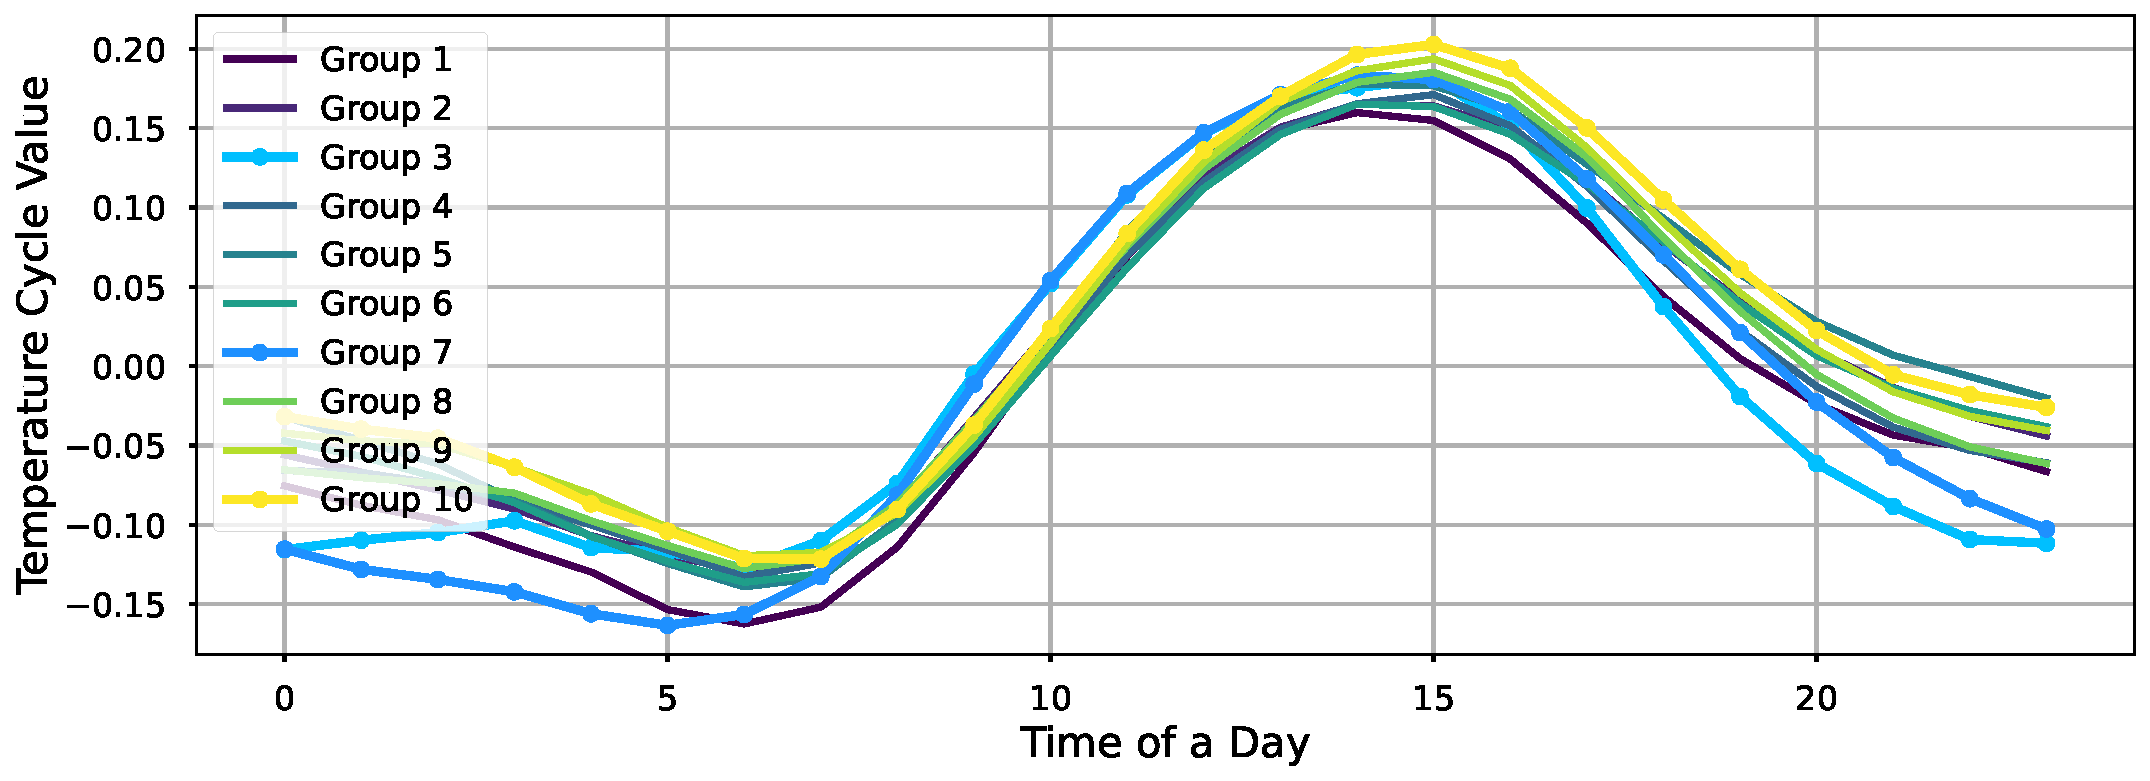
\includegraphics[width=1.0\linewidth]{resources/cycle.pdf}
    \vspace{-2.5em}
    \caption{Daily thermal cycle for different station groups.}
    \label{fig:cycle}
\end{figure}

\textbf{Thermal cycle modeling.} We first visualize the learned daily thermal cycle for different station groups in our cycle learning block. In Figure \ref{fig:cycle}, we observe that the learned daily temperature patterns show that stations warm up before 15:00 PM, cool down at night, and reach their lowest temperatures just before sunrise. This aligns well with the natural temperature patterns typical of Seoul, which has a temperate monsoon climate. Additionally, the differences observed between various station groups accurately reflect the thermal cycle variations in regions with different environments. For example, stations situated in dense urban areas (\underline{Group 10}) consistently show higher regional temperatures, indicating an increased heat risk, while regions with water bodies (\underline{Group 7}) and greenbelt (\underline{Group 3}) display distinctive temperature cycles. These results and observations demonstrate that the thermal cycle learning block, along with our decomposition-based framework, effectively captures clear and precise thermal cycles from noisy historical temperature data.

\begin{figure}[!t]
    \centering
    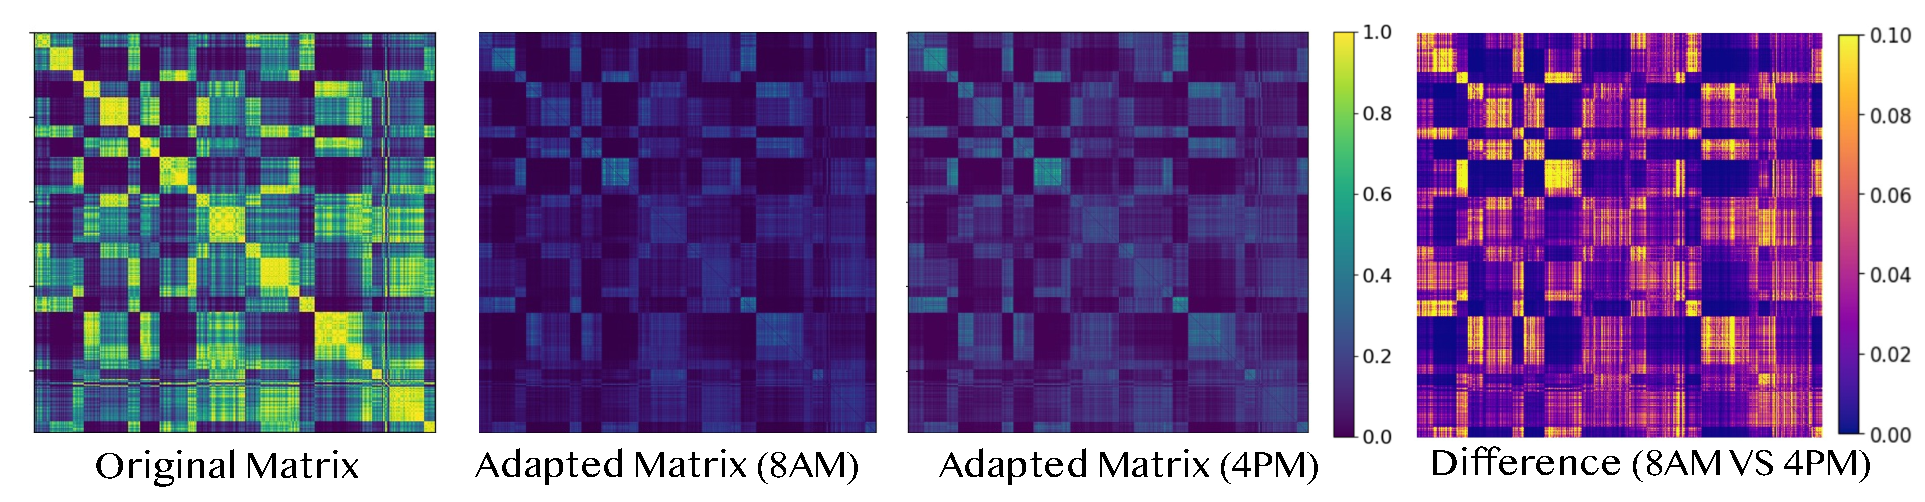
\includegraphics[width=1.0\linewidth]{resources/flow.pdf}
    \vspace{-2em}
    \caption{Adapted adjacent matrix for thermal flow modeling at different time steps.}
    \label{fig:flow}
    \vspace{-1em}
\end{figure}


\textbf{Thermal flow modeling.} In our decomposition-based framework, we utilize spatial graph convolution to model the mechanics of heat flow and introduce a dynamic adaptive adjacency matrix to capture its anisotropy at different time periods. We visualized both the original distance-based adjacency matrix and the learned adaptive matrix for thermal heat flow during the morning, noon, and evening. The differences between the original and learned matrices indicate the anisotropy of spatial heat flow learned by our model, as the vanilla distance-based adjacency matrix is isotropic. Additionally, it is evident that our learned matrix exhibits variations across different time periods, which corresponds well with the dynamic mechanics of thermal flow.

\subsection{Ablation Study (RQ4)}
\begin{figure}[!b]
    \centering
    \vspace{-1em}
    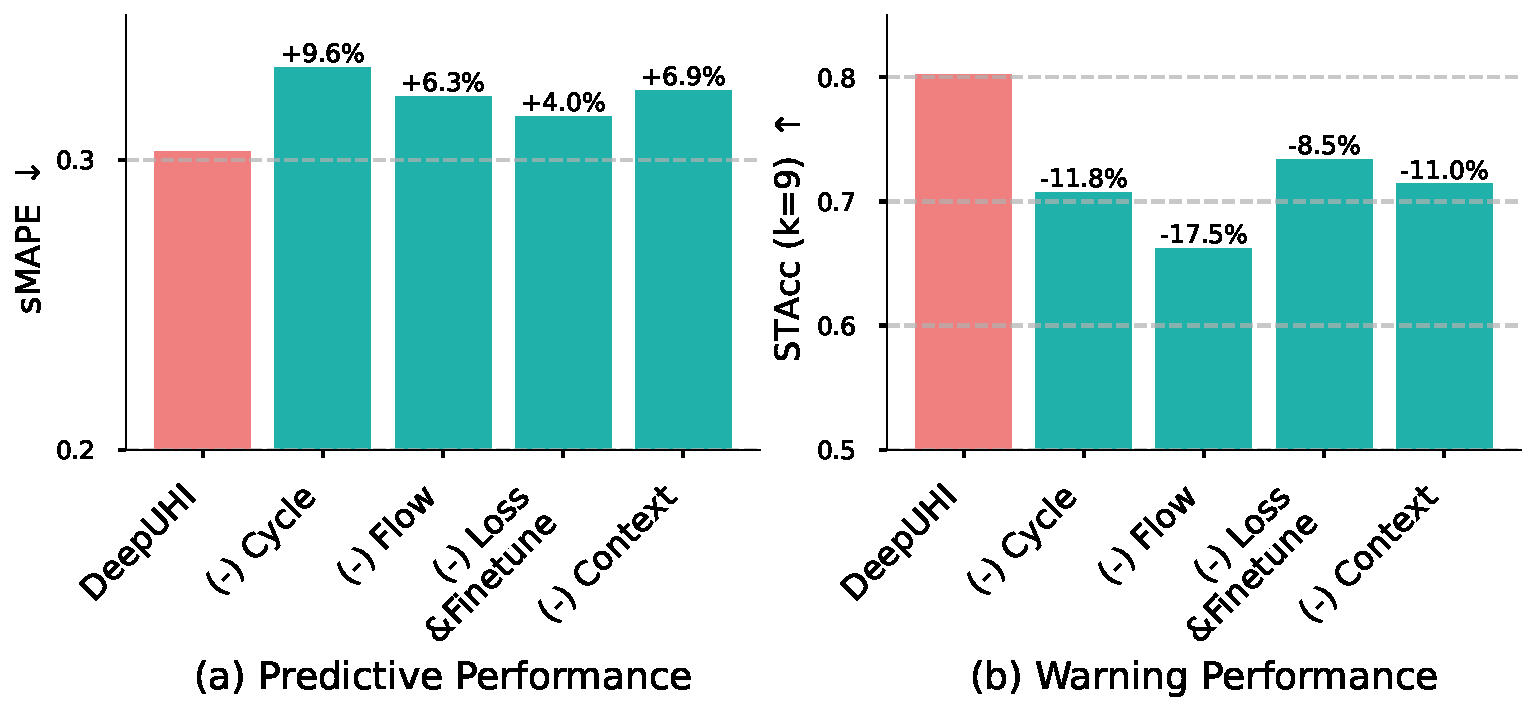
\includegraphics[width=1\linewidth]{resources/ablation.pdf}
    \vspace{-2em}
    \caption{Ablation study on prediction and warning tasks.}
    \label{fig:ablation}
\end{figure}
To investigate the impact of each proposed component of our framework on its performance, we developed the following model variants for an ablation study:
\begin{itemize}[leftmargin=*]
    \item \textbf{(-) Cycle}. This variant removes the thermal cycle learning block and includes no daily cycle decomposing in the framework.
    \item \textbf{(-) Flow}. This variant removes the heat flow learning block and uses a 3-layer MLP for regression.
    \item \textbf{(-) Loss \& Fine-tune}. This variant replaces the variant-aware loss with MSE loss and drops the fine-tuning training strategy.
    \item \textbf{(-) Context}. This variant drops the contextual features for region clustering and regional relations adapting.
\end{itemize}

We report the ablation results of \model and its variants on both temperature prediction and urban heat island (UHI) warning performance in Figure~\ref{fig:ablation}. In summary, our findings are as follows: 1) For the predictive task, thermodynamic modeling plays the most significant role. This indicates that clear daily pattern information can greatly enhance the model's performance in prediction. However, for the warning task, thermal flow modeling is crucial for maintaining high performance. Warning tasks require a deeper understanding of spatio-temporal dynamics, making the dynamic relationship modeling process essential for comprehending complex thermal flows. 2) The variation-aware loss and fine-tuning strategy can improve performance in both tasks to a similar extent. 3) Contextual features can enhance model performance in both tasks; however, if they are excluded, the self-adaptive version of \model still yields satisfactory results.

